\documentclass[12pt, letterpaper]{article}
\usepackage[utf8]{inputenc}
\usepackage{minted}
\usepackage{graphicx} %package to manage images
\graphicspath{ {images/} }
\usepackage{hyperref}

\thispagestyle{plain}
\begin{document}
\begin{center}
    \Large
    \textbf{Análise comparativa de ferramentas de Workflow para Ruby}
    
    \vspace{0.4cm}
    \large
    Engenharia de Processos e Requisitos
    
    \vspace{0.4cm}
    \textbf{Eduardo Mauricio Barbiero}
    
    \vspace{0.4cm}
    {Dezembro de 2015}
    
    \vspace{0.9cm}
    \textbf{Resumo}
\end{center}

\par
Análise comparativa entre dois FrameWorks desenvolvidos com Ruby, para auxiliar no Fluxo de trabalho de um determinado negócio. Será feita uma breve descrição sobre os dois frameworks "Workflow" e "Rails Workflow", que possuem algumas particularidades e demonstrado em forma de tabela a representação de funcionalidades e diferenças. 

\section{Workflow}

Workflow é uma API inspirada na "máquina de estados finitos" para a modelagem e interagir com o que temos a tendência de se referir como "fluxo de trabalho".

Uma grande remeça de informaçõe sobre o negócio, tende a envolver conceitos de fluxo de trabalho, bem como, essa biblioteca tende a expressar que esses conceitos sejam o mais claro possível. É utilizada uma terminologia semelhante encontrada na "teoria de máquina de estado".

Um fluxo de trabalho possui sempre um estado. Ele só pode estar em um estado de cada vez, porém, quando ele muda de estado, chamamos isso de transição. As transições de um evento, ocorrem de modo que cada transição ocorra, onde caso haja alguma falha na execução dessa transição, seja executado uma outra remessa de código, que possa ou não corrigir esse problema. Desse modo, esses transições podem gerar vários eventos, e qualquer evento pode gerar uma outra transição ou uma nova ação.

Aplicando esses conceitos a um caso, digamos que uma cidade possui alguns problemas e devem ser resolvido com alguns passos, até que chegue a um determinado setor de uma empresa. Dessa forma, um problema é diagnosticado, passado a uma analista de problemas até chegar ao responsável pelo setor. Após isso, deve ser enviada a uma determinada área para execução ou reparação do problema, vejamos na utilização da API:

\begin{minted}
[
frame=lines,
framesep=2mm,
baselinestretch=1.2,
fontsize=\footnotesize,
]
{ruby}
 class Problemas
  include Workflow
  workflow do
    state :new do
      event :submit, :transitions_to => :aguardando_revisao
    end
    
    state :aguardando_revisao do
      event :review, :transitions_to => :sendo_revisado
    end
    
    state :sendo_revisado do
      event :accept, :transitions_to => :accepted
      event :reject, :transitions_to => :rejected
    end
    
    state :accepted
    state :rejected
  end
end
\end{minted}
Nesse caso, o uso ficaria dessa forma: 
\begin{minted}
[
frame=lines,
framesep=2mm,
baselinestretch=1.2,
fontsize=\footnotesize,
]
{ruby}
problema = Problemas.new
problema.accepted? # => false
problema.new? # => true
\end{minted}

Ou seja, é verificado se o problema foi aceito, e verifica se é um evento novo.

Uma outra forma de verificar esse status, é chamando o objeto "\texttt{current\_state}" que retorna um objeto de estados do workflow atual.

\begin{minted}
[
frame=lines,
framesep=2mm,
baselinestretch=1.2,
fontsize=\footnotesize,
]
{ruby}
problema.current_state
=> #<Workflow::State:0x7f1e3d6731f0 @events={
  :submit=>#<Workflow::Event:0x7f1e3d6730d8 @action=nil,
    @transitions_to=:aguardando_revisao, @name=:submit, @meta={}>},
  name:new, meta{}
\end{minted}  

Agora precisamos saber, se o problema foi aceito, e onde se encontra nossa review:

\begin{minted}
[
frame=lines,
framesep=2mm,
baselinestretch=1.2,
fontsize=\footnotesize,
]
{ruby}
problema.current_state < :accepted
=> true
problema.current_state >= :accepted
=> false
problema.current_state.between? :aguardando_revisao, :rejected
=> true
\end{minted}  

Nesse caso, podemos observar, que ele se encontra "\texttt{aguardando\_revisao}", e desse modo ele ainda é "rejeitado". 

Agora nós podemos chamar o evento "submit", que faz a transição para o estado "\texttt{aguardando\_revisao}":

\begin{minted}
[
frame=lines,
framesep=2mm,
baselinestretch=1.2,
fontsize=\footnotesize,
]
{ruby}
problema.submit !
problema.aguardando_revisao? # = > True
\end{minted}  

Esses eventos, são na verdade métodos de instancia de um fluxo e trabalho, que dependendo do estado onde você está, ele vai conter um conjunto de eventos diferentes para serem usandos e para auxiliar na transição para outros estados.

É fácil verificar se uma certa transição foi feita, a partir do evento atual, basta verificar pelo método "\texttt{problema.can\_submit?}", se essa transição foi submetida do estado atual.

\section{Rails WorkFlow}

Rails Workflow permite que você organize a sua lógica de negócios do aplicativo juntando operações pelo usuário e automatizar processos. Você pode configurar, criar e gerenciar processos para construir facilmente os sistemas de gerenciamento de projetos, vendas/sistemas de aprovisionamento de produtos, ERP, CMS, etc.  Rails Workflow é feito em Rails e pode ser montado em qualquer aplicação Rails.

Todos os processos, configurações, operações e seus dados são mantidos para fins de processamento e de apoio. Essa Engine tem UI para configurar os modelos de processo e gerenciar os processos existentes.

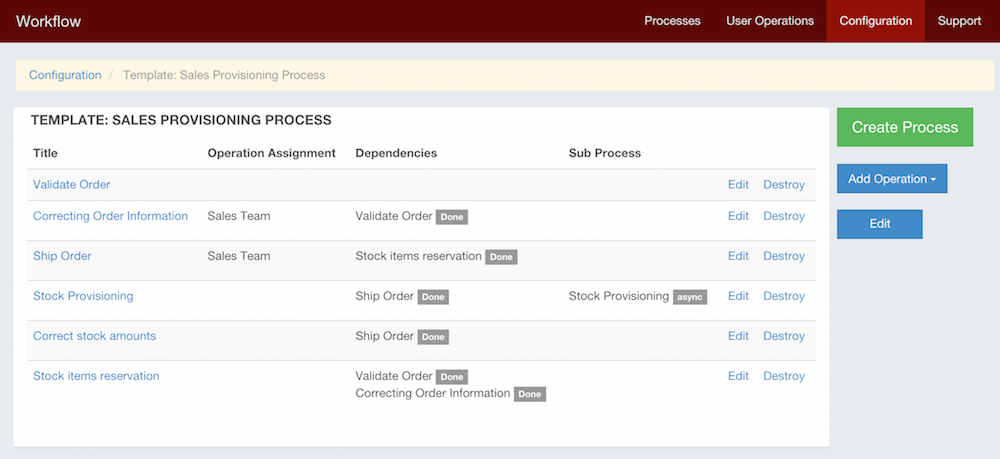
\includegraphics[width=13cm, height=7cm]{railsworkflow}

\par
Rails Workflow é de fácil instalação e utilização, o que torna esse camada de instalação/desenvolvimento mais rápida.

\begin{minted}
[
frame=lines,
framesep=2mm,
baselinestretch=1.2,
fontsize=\footnotesize,
]
{ruby}
gem 'rails_workflow', '0.3.5'

#config/application.rb
require 'rails_workflow'

#routes.rb
Rails.application.routes.draw do
mount RailsWorkflow::Engine => '/workflow', as: 'workflow'
end

rails generate rails_workflow:install
\end{minted} 
\par

O desenvolvimento dessa gem foi iniciada após a liberação Rails 4, assim todas as atividades de desenvolvimento está focada para suportar essa versão do Ruby on Rails.

Rails workflow gem depende seguintes gems para funcionamento:
\begin{itemize}
  \item bootstrap-rails-engine
  \item devise
  \item \texttt{will\_paginate}
  \item sidekiq
  \item slim-rails
  \item jquery-rails
  \item jquery-ui-rails
  \item draper
  \item Utilizar Ruby 2.
\end{itemize}

É resposável pela iniciação do fluxo de trabalho:
\begin{minted}
[
frame=lines,
framesep=2mm,
baselinestretch=1.2,
fontsize=\footnotesize,
]
{ruby}
RailsWorkflow::ProcessManager.build_process template_id, context
RailsWorkflow::ProcessManager.start_process template_id, context
\end{minted} 
Onde, "\texttt{template\_id}" é um id de sua ProcessTemplate e "context" é um hash, por exemplo \big\{resource: produto\big\}
\subsection{Operação de template}
\par
Operação de template é responsável por detectar se a operação deve ser criada(dependências de resolução) e para a construção de operação.
\begin{minted}
[
frame=lines,
framesep=2mm,
baselinestretch=1.2,
fontsize=\footnotesize,
]
{ruby}
# Verifica se o processo pode comecar.
process.can_start?

# Inicia processo
process.start

# verifica se o processo ja foi completo:
# completed - caso tenha terminado.
# incomplete - caso nao tenha terminado.
process.can_complete?

# Operacoes que ainda nao foram concluidas, eles podem ser:
# in_progress, waiting, error, etc.
# Operacoes completas - done, skipped, canceled.
process.incompleted_operations

# Tentando construir nova operacao, ou para finalizar a operacao.
process.operation_complete(operation)

# Processo completo.
process.complete

\end{minted}  
\subsection{Operações}
\begin{minted}
[
frame=lines,
framesep=2mm,
baselinestretch=1.2,
fontsize=\footnotesize,
]
{ruby}
# Verifica se a operacao pode ser iniciada
# if operation_status = NOT_STARTED.
operation.can_start?

# Ira iniciar a operacao
operation.start

# A partir daqui, voce pode iniciar o desenvolvimento, ou seja, pode adicionar seu codigo
operation.execute

# Verifica se esta completa
operation.completed?

# Verifica se possui processos filhos e seu status
operation.can_complete?

# Utilizado quando o usuario fizer alguma acao e resultar no fim dessa operacao, ira executar o codigo
operation.on_complete

\end{minted}  
Esses são os principais passos para verificação e mudança de estado de uma operação
\subsection{Operações de Usuário}
Há métodos específicos para operações com base em usuários, que são importantes:
\begin{minted}
[
frame=lines,
framesep=2mm,
baselinestretch=1.2,
fontsize=\footnotesize,
]
{ruby}

# Verifica se operacao pode ser atribuida a este usuario
operation.can_be_assigned? user

# Verifica se foi atribuida a este usuario
peration.assigned? user

# Restaura a operacao inicial atribuida a funcao ou grupo
operation.cancel_assignment user

# Atribui operacao a este usuario
operation.assign user

\end{minted} 

\newpage
\section{Comparação}
A seguir será feita uma comparação entre as duas tecnologias.
\begin{center}
\begin{tabular}{|l|l|l|l|l|l|l|l|l|}
\hline
               & \scriptsize{Ruby}  & \scriptsize{Maleável} & \scriptsize{Rastreável} & \scriptsize{Interface} & \scriptsize{Tutoriais} & \scriptsize{Escalabilidade} & \scriptsize{Processos} \\ \hline
\scriptsize{WorkFlow}       & 1.9.x & -1       & +1         & -1        & +1        & -1             & -1        \\ \hline
\scriptsize{Rails Workflow} & 2.x   & +1       & +1         & +1        & -1        & +1             & +1        \\ \hline
\end{tabular}
\end{center}

\newpage
\section{Conclusão}

\par
Pelo fato do gem Workflow ser extremamente simples de ser usado e aplicado, torna-se uma boa escolha, quando se trata de um sistema de não tanta regra de negócio sobre o fluxo de trabalho. Ao contrário da Rails Workflow que traz uma ótima interface, onde pode ser acompanhado em qual etapa encontra-se o fluxo, sem muito código digitado e podendo fazer essas alterações em tempo real, e fazer requisições assíncronas e síncronas.
\par
Com base nisso, vale se destacar que de tal forma o programador deve se adequar no que realmente se precisa e a que melhor se encaixa na regra de negócio. A robustez da Rails Workflow e facilidade de mutação, ou a simplicidade da Workflow para desenvolvimento de uma api/app de simples manutenção.

\newpage
\section{Referências}
\url{https://github.com/geekq/workflow}\break
\url{https://github.com/madzhuga/rails_workflow}\break
\url{http://www.rails-workflow.com/}


\pagenumbering{arabic}

\end{document}